\documentclass[11pt,a4paper]{article}

\usepackage[margin=1in]{geometry}
\usepackage{titlesec}
\usepackage{enumitem}
\usepackage{hyperref}
\usepackage{parskip}
\usepackage{graphicx}
\usepackage{float}
\usepackage{booktabs}
\usepackage{amsmath}

\hypersetup{colorlinks=true, linkcolor=blue, urlcolor=blue}

\titleformat{\section}{\large\bfseries}{\thesection}{0.5em}{}
\titleformat{\subsection}{\normalsize\bfseries}{\thesubsection}{0.5em}{}
\setlist{leftmargin=1.4em, topsep=2pt, itemsep=2pt}

\title{\vspace{-1.5cm}\textbf{PKCERT AI \& Software Development Internship \\ Task 15: Model Persistence \& Mini-Project}}
\author{Abdullah Amir}
\date{AI and Software Development \\ 22 July 2026}

\begin{document}

\maketitle
\vspace{-0.8cm}

This report covers the theory and the results. The full code, outputs and plots live in
the notebook \texttt{model\_persistence.ipynb}. The mini-project dataset is the
\textbf{UCI Cleveland Heart Disease} dataset (303 patients), not used in any earlier
task. A Logistic Regression and a Random Forest are trained and compared, the better one
is saved with both \textbf{pickle} and \textbf{joblib}, and the two formats are checked
for correctness, size and speed.

% ----------------------------------------------------------------
\section*{Part C: Dataset Selection, EDA \& Preprocessing (Mini-Project)}

\textbf{What the features are.} Each row is one patient: 13 clinical features -- 6
numeric (\texttt{age}, \texttt{trestbps}, \texttt{chol}, \texttt{thalach},
\texttt{oldpeak}, \texttt{ca}) and 7 categorical (\texttt{sex}, \texttt{cp},
\texttt{fbs}, \texttt{restecg}, \texttt{exang}, \texttt{slope}, \texttt{thal}) -- and a
target of whether angiography showed more than 50\% coronary narrowing.

\textbf{Missing values, checked rather than assumed away.} Only \texttt{ca} (5 missing)
and \texttt{thal} (2 missing) have gaps, 2.3\% of rows. Dropping those 7 rows shifts the
positive rate from 45.5\% to 45.9\% -- negligible -- but median/most-frequent imputation
is used anyway, since it preserves the full 303 rows and is the more complete
demonstration of the preprocessing step the task asks for.

\begin{figure}[H]
    \centering
    
\includegraphics[width=0.95\textwidth]{figures/01_dataset_overview.png}
    \caption{Left: the target is close to balanced, 45.5\% positive. Right: patients with
    disease skew older (median 58 vs 52), as expected, but the overlap is substantial --
    age alone is a weak signal.}
\end{figure}

\begin{figure}[H]
    \centering
    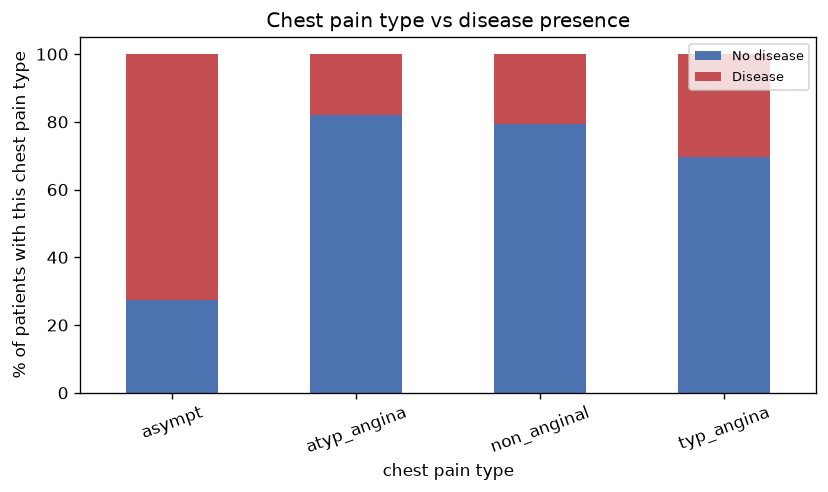
\includegraphics[width=0.72\textwidth]{figures/02_chest_pain_vs_target.png}
    \caption{Chest pain type against disease presence.}
\end{figure}

\textbf{A counterintuitive detail worth flagging.} \texttt{asympt} (asymptomatic -- no
chest pain reported) has the \emph{highest} disease rate of any category, 72.7\%, while
every named type of pain has a \emph{lower} rate (\texttt{typ\_angina} 30.4\%,
\texttt{non\_anginal} 20.7\%, \texttt{atyp\_angina} 18.0\%). The absence of the symptom
you would expect to see is the strongest single signal in this feature -- exactly the
kind of relationship that is easy to miss without checking the crosstab directly.

\textbf{Split and preprocessing.} An 80/20 stratified split (242 train / 61 test rows).
A \texttt{ColumnTransformer} imputes and standard-scales the numeric columns and imputes
and one-hot encodes the categorical ones, wrapped in a single \texttt{Pipeline} per
model so that preprocessing travels with the model when it is saved.

\subsection*{Model selection}

\begin{table}[H]
\centering
\small
\setlength{\tabcolsep}{4.5pt}
\begin{tabular}{lrrrrr}
\toprule
\textbf{Model} & \textbf{CV ROC-AUC} & \textbf{Test Acc} & \textbf{Precision} & \textbf{Recall} & \textbf{Test ROC-AUC} \\
\midrule
Logistic Regression & 0.9017 $\pm$ 0.031 & \textbf{0.8525} & \textbf{0.8519} & \textbf{0.8214} & \textbf{0.9275} \\
Random Forest (300 trees) & 0.9037 $\pm$ 0.029 & 0.8033 & 0.8333 & 0.7143 & 0.8837 \\
\bottomrule
\end{tabular}
\caption{5-fold cross-validated ROC-AUC on the training set, then held-out test metrics.}
\end{table}

\begin{figure}[H]
    \centering
    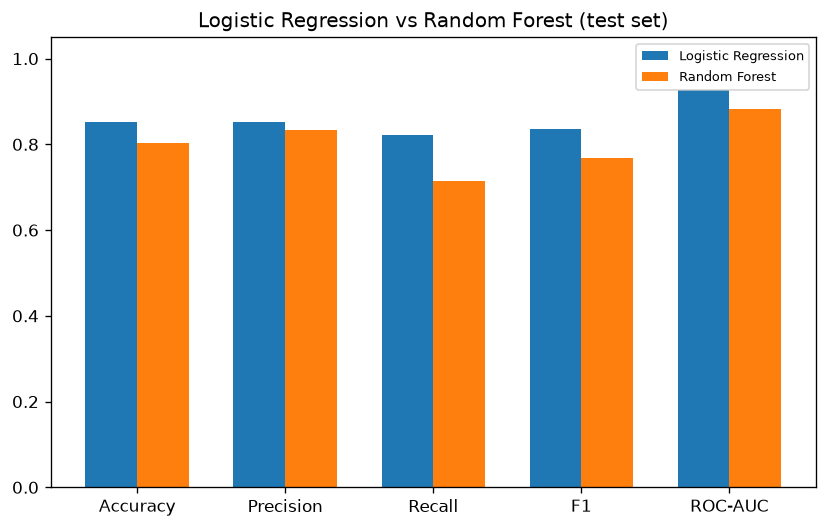
\includegraphics[width=0.68\textwidth]{figures/03_model_comparison.png}
    \caption{Logistic Regression vs Random Forest on every test-set metric.}
\end{figure}

\textbf{The simpler model won, and the two cross-validation scores explain why it is not
a fluke.} In cross-validation the two models are essentially tied (0.9017 vs 0.9037), but
on the held-out test set Logistic Regression pulls ahead on every metric (ROC-AUC 0.9275
vs 0.8837). With only 242 training rows, a 300-tree Random Forest has considerably more
capacity to fit sampling noise than a linear model does -- a concrete instance of the
bias-variance tradeoff rather than a coincidence of one split. Logistic Regression is
the model saved and persisted below.

\begin{figure}[H]
    \centering
    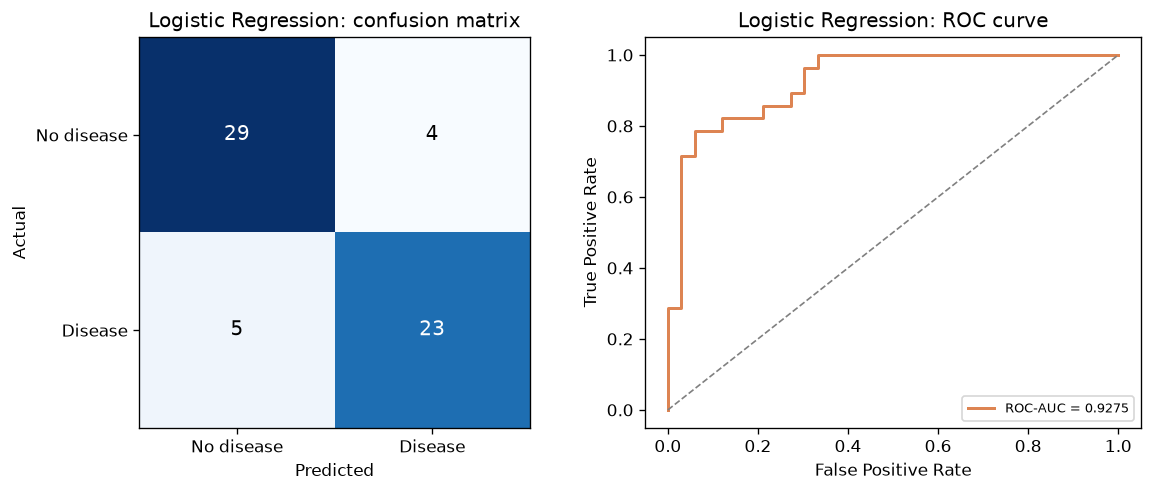
\includegraphics[width=0.95\textwidth]{figures/04_confusion_roc.png}
    \caption{The chosen model's confusion matrix and ROC curve on the test set.}
\end{figure}

\begin{figure}[H]
    \centering
    
\includegraphics[width=0.68\textwidth]{figures/05_feature_importance.png}
    \caption{Random Forest feature importance, shown for reference even though Logistic
    Regression was the model kept. \texttt{thal\_normal}, \texttt{thalach} (max heart
    rate) and \texttt{oldpeak} (ST depression) lead.}
\end{figure}

% ----------------------------------------------------------------
\section*{Part A: Saving Trained Models}

The chosen Logistic Regression pipeline -- preprocessing and classifier together -- was
saved two ways:

\begin{table}[H]
\centering
\begin{tabular}{lr}
\toprule
\textbf{Format} & \textbf{File size} \\
\midrule
\texttt{pickle} (\texttt{heart\_model.pkl}) & 3,754 bytes \\
\texttt{joblib} (\texttt{heart\_model.joblib}) & 5,930 bytes \\
\bottomrule
\end{tabular}
\end{table}

% ----------------------------------------------------------------
\section*{Part B: Loading \& Verifying Models}

Both files were loaded back into fresh Python objects and checked against the original
in-memory model's predictions on the test set, both the hard labels and the underlying
probabilities.

\textbf{Both round-trips are bit-for-bit identical to the original}: predicted labels
match exactly and predicted probabilities match to floating-point precision
(\texttt{numpy.allclose}), for both the pickle-loaded and the joblib-loaded copy.
Serialization lost nothing.

\subsection*{pickle vs joblib, checked rather than recited}

The common claim is that joblib is more efficient for scikit-learn models because of
how it handles the large numpy arrays inside them. Logistic Regression barely has any
(a handful of coefficients), so the same save/load/size/time comparison was repeated on
the 300-tree Random Forest -- orders of magnitude more numpy array data -- to test
whether that claim actually holds.

\begin{table}[H]
\centering
\begin{tabular}{lrrrr}
\toprule
& \multicolumn{2}{c}{\textbf{Logistic Regression (small)}} & \multicolumn{2}{c}{\textbf{Random Forest (300 trees)}} \\
\textbf{Format} & \textbf{Size} & \textbf{Load time} & \textbf{Size} & \textbf{Load time} \\
\midrule
pickle & 3,754 B & 0.12 ms & 2,169,710 B & 4.58 ms \\
joblib & 5,930 B & 0.63 ms & 2,195,451 B & 23.21 ms \\
\bottomrule
\end{tabular}
\caption{Same comparison, small model and large model.}
\end{table}

\begin{figure}[H]
    \centering
    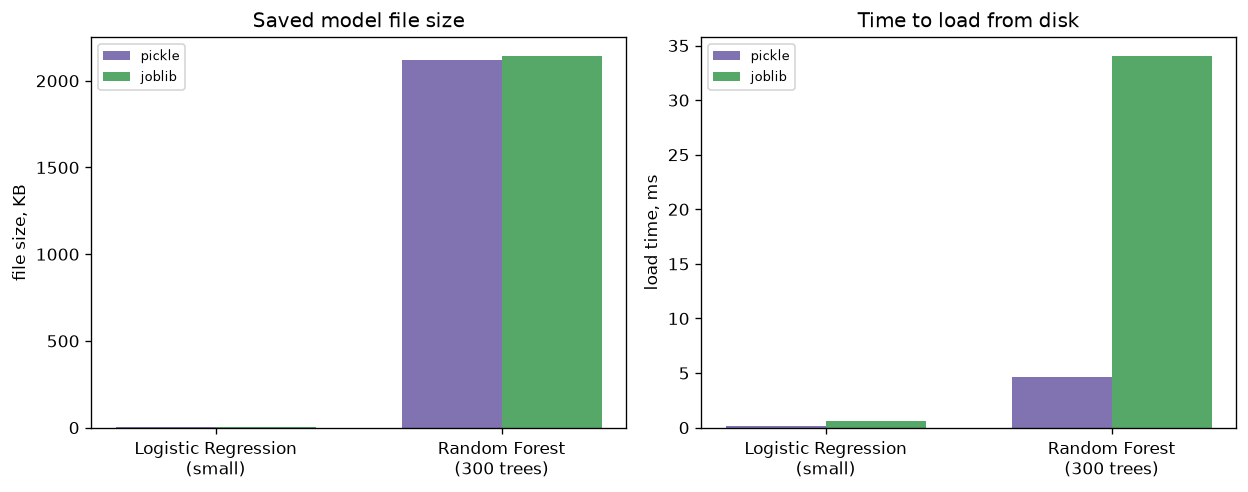
\includegraphics[width=0.95\textwidth]{figures/06_persistence_comparison.png}
    \caption{pickle vs joblib, file size and load time, on both models.}
\end{figure}

\textbf{The result contradicts the common claim, on both models.} pickle was smaller and
faster than joblib for the small Logistic Regression \emph{and} for the 2MB Random
Forest -- joblib was 58\% larger for the small model and still 1.2\% larger for the
large one, and pickle loaded 2--5x faster in both cases.

The likely reason is \textbf{PEP 574} (Python 3.8+): pickle protocol 5 added native
out-of-band buffer support for numpy arrays, closing most of the efficiency gap joblib
was originally built to fix back in 2008, long before protocol 5 existed. On a modern
Python interpreter, plain pickle is often just as compact and avoids joblib's own
dispatch overhead.

\textbf{What joblib still does that pickle does not:} a one-argument \texttt{compress=}
parameter for gzip-style compression without wrapping the file handle manually, and
\texttt{mmap\_mode} for loading a huge array from disk without reading all of it into
RAM at once -- useful for models far larger than either one tested here. It also remains
scikit-learn's own documented recommendation for persisting estimators, largely for
these convenience features rather than raw size or speed.

\textbf{When to use each.} Plain \texttt{pickle} for small models and general Python
objects where no extra dependency is wanted; \texttt{joblib} when a model is large
enough that \texttt{compress=} or \texttt{mmap\_mode} will matter in practice, or simply
to follow scikit-learn's own convention.

\textbf{A caveat worth stating plainly.} Never unpickle a model file from an untrusted
source. Both \texttt{pickle.load} and \texttt{joblib.load} execute arbitrary code
embedded in the file by design -- that is what lets them reconstruct arbitrary Python
objects -- so a malicious \texttt{.pkl} or \texttt{.joblib} file is a code-execution
risk, not merely a data file.

% ----------------------------------------------------------------
\section*{Part D: Model Saving \& Documentation}

\textbf{Pipeline summary.} Loaded the UCI Cleveland Heart Disease dataset (303 patients,
a dataset unused in any earlier task) $\rightarrow$ checked missing values (2.3\% of
rows, \texttt{ca}/\texttt{thal} only) and confirmed dropping them barely shifts the class
balance $\rightarrow$ built a \texttt{ColumnTransformer} that imputes and scales numeric
features and imputes and one-hot encodes categorical ones $\rightarrow$ trained and
cross-validated Logistic Regression and a 300-tree Random Forest $\rightarrow$ selected
Logistic Regression on held-out ROC-AUC (0.9275 vs 0.8837) $\rightarrow$ saved it with
both pickle and joblib $\rightarrow$ loaded both back and verified bit-for-bit identical
predictions $\rightarrow$ repeated the save/load comparison on the larger Random Forest
to test whether joblib's usual efficiency claim holds.

\textbf{Key findings.}
\begin{enumerate}
    \item Asymptomatic patients have the \emph{highest} disease rate (73\%) of any chest
    pain category -- the absence of a symptom outranks its presence as a signal.
    \item The simpler model beat the more flexible one on every held-out metric despite
    being statistically tied in cross-validation -- a concrete instance of the
    bias-variance tradeoff on a 242-row training set.
    \item Both saved-model round-trips reproduced the original predictions exactly, with
    no loss of precision from serialization.
    \item Contrary to the common claim, \textbf{pickle beat joblib on both size and
    speed} for both a tiny model and a 2MB one on this machine -- a reminder that
    ``joblib is more efficient'' is a claim worth re-checking against the current Python
    version rather than repeating from memory.
\end{enumerate}

\textbf{Challenges faced.} The dataset's raw target is a five-level severity scale
(0--4) and had to be collapsed to binary ($>$50\% narrowing or not) to match how it is
almost universally used in classification benchmarks. The anonymised OpenML mirror
exposes columns only as \texttt{V1}...\texttt{V13}, so matching them back to their real,
documented clinical names required cross-referencing the original UCI column order
rather than trusting the mirror alone -- the same care that mattered for Day 14's Bank
Marketing dataset. The pickle-vs-joblib size result was the opposite of what is commonly
repeated online, which made it tempting to assume a bug in the benchmark; verifying it
on a second, much larger model before trusting it was the only way to be sure it was a
real result and not noise from one small file.

\textbf{Conclusion.} The thread running through this task is that persistence is not a
detail to bolt on after modelling is finished -- it is where a model actually becomes
useful outside the notebook that trained it, and both format choice and integrity
deserve the same scepticism applied everywhere else in this internship. Saving is easy;
what is worth checking is whether the thing you load back is truly the thing you saved,
and whether the received wisdom about how to save it still holds.

\vspace{0.4cm}
\noindent The notebook and README are on GitHub: {\small\scalebox{0.72}[1]{\url{https://github.com/AbdullahAmir06/ai-internship-abdullahamir}}}

\end{document}
